\documentclass[a4paper,10pt]{article}
%\documentclass[a4paper,10pt]{scrartcl}
\usepackage[spanish]{babel}
\usepackage[utf8]{inputenc}
\usepackage{amssymb, amsmath, amsbsy}
\usepackage{cancel} % para tachar
\usepackage{mathdots} % para el comando \iddots
\usepackage{mathrsfs} % para formato de letra
\usepackage{stackrel} % para el comando \stackbin
\usepackage{graphicx}
\graphicspath{ {images/} }

\title{Describir los métodos geométrico, algebraico y desacoplo cinemático}
\author{Gutiérrez Muñoz José de Jesús \\ 7 - A \\ Ing. Mecatrónica}
\date{22- Octubre - 2019}

\begin{document}
\maketitle
\centering Metogo Geométrico

\begin{itemize}
\item Es un método no sistemático que utiliza las relaciones geométricasparaobtenerlaposicióndelextremodelrobotparaobtenerlaposicióndelextremodelrobot.
\item Normalmente se emplea para la obtención de la posición y no de laorientación.
\item Se usan en robots de pocos grados de libertad.
\end{itemize}

\begin{center}
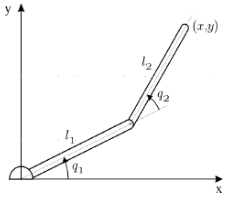
\includegraphics[width=0.7\textwidth]{imagen1.png}
\end{center}

\begin{center}
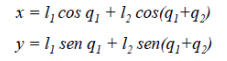
\includegraphics[width=0.7\textwidth]{Imagen.png}
\end{center}

\pagebreak

\centering Desacoplo Cinemático.

\centering Resolución mediante el desacoplo cinemático 

\begin{itemize}

\item Habitualmente los tres último ejes del robot se cortan en un punto

\item La finalidad de estos es lograr la orientación de la herramienta, aunque como consecuencia de su movimiento tengan un efecto ligero sobre la posición.

\item Con la primera condición se puede simplificar enormemente el proble macinemático para 6 gdl, dado que la obtención de este punto de intersección es una operación sencilla. punto de intersección es una operación sencilla. 

\item Este punto dependerá sólo de los 3 primeros gdl, por lo que su obtención es asequible.
\end{itemize}


\begin{center}
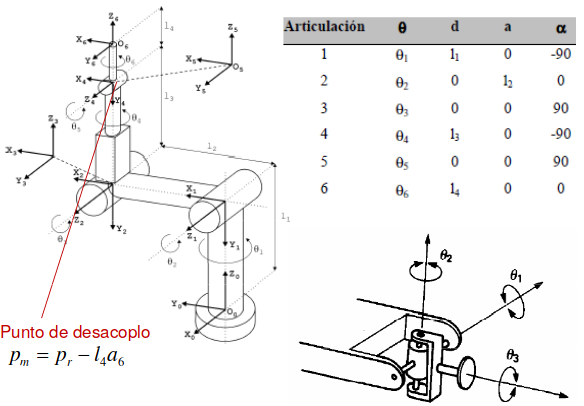
\includegraphics[width=0.7\textwidth]{imagen3.png}
\end{center}

Mediante alguno de los métodos anteriores se obtien en los valores de $q1, q2 y q3$ ¿Qué hacemos con el resto? de $q1, q2 y q3$. ¿Qué hacemos con el resto?


Nos centramos exclusivamente en la orientación por simplicidad, y aplicamos un método análogo al basado en  las matrices homogéneas:

\hfill

$^0R_6 = ^0R_3 \ ^3R_6 = [n \ o \ a]

^3R_6 = ^3R_4 \ ^4R_5 \ ^5R_6 = (^0R_3)^-1 [n \ o \ a] = (^0R_3)^T [n \ o \ a]

^4R_5 \ ^5R_6 = (^3R_4)^T \ (^0R_3)^T \ [n \ o \ a] 

\begin{center}
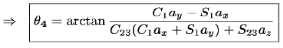
\includegraphics[width=0.7\textwidth]{imagen5.png}
\end{center}

^5R_6 = (^4R_5)^T \ (^3R_4)^T \ (^0R_3)^T \ [n \ o \ a]

\begin{center}
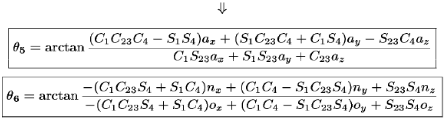
\includegraphics[width=0.7\textwidth]{imagen4.png}
\end{center}
$

\centering Metodo algebraico

\hfill

El desarrollo de la cinemática directa de un robot da como resultado un conjunto de ecuaciones no lineales que describen el comportamiento de la pose del efector final. Los métodos algebraicos consistenen igualar estas ecuacionesa la posición y orientación deseada, para después hacer una manipulación   matemática   que   permita   despejar   cada   una   de   las variables   de   las juntas $(q1,q2,...,qn)$.

\hfill

Siempre  que  sea  posible  se  recomienda  resolver  lacinemática  inversa  algebraicamente,  ya  que éste método ofrecelasventajasde ser robusto, requerir en general menor costo computacional, y  por  lo  tanto  obtener  resultadosmás  rápido,  además  de  que  permite  encontrar  todas  las soluciones  posibles.  Sin  embargo,  tienela  desventajade  no  ser  un  método fácil,  ya  quepara algunos robots encontrar las relacionesnecesarias es extremadamente complicado, debido a que éstas suelen ser ecuaciones no lineales.En estos casos es necesarioacercarse al problema de otras formas, como métodos numéricos o heurísticos.

\hfill

Existen  dos  métodos  para  resolver  la  cinemática  inversa  de  cualquier  robot  algebraicamente siempre  que  la  cadena  cinemática  del  robot  cumpla  características  específicas:  El  método geométrico se usa sólo para robots de pocos grados de libertad y el desacoplamientocinemático para robots de 6 GDL que poseen una muñeca esférica.

\end{document}
